\section{Leptons as Standing Phase Oscillations}

In GCFT, leptons are not elementary particles but topological phase locks in the coherence field~$\Xi$. Their stability and mass arise from compression thresholds and torsional configurations, and their charge emerges from curl biases in the field.

\begin{table}[ht]
\centering
\begin{tabular}{lcc}
\hline
\textbf{Property} & \textbf{Standard Model} & \textbf{GCFT} \\
\hline
Particle ontology & Point-like & Phase-locked field knot \\
Charge quantization & Imposed & Topological winding \\
Mass origin & Higgs coupling & Field compression \\
Stability & Assumed & Knot curvature \\
Decay & Weak force mediation & Knot decoherence \\
\hline
\end{tabular}
\caption{Lepton properties: Standard Model vs. GCFT.}
\label{tab:lepton_compare}
\end{table}

\subsection{\texorpdfstring{Electron: Stable $\Xi$ Curl Node}{Electron: Stable Xi Curl Node}}

The electron corresponds to a persistent knot in $\nabla \times \nabla \arg(\Xi)$---a localized torsional resonance with a field retention threshold of 4.7\,eV. Its long-lived nature results from the stability of this resonance under field drift. The electron is the archetype of a stable $\Xi$-phase curl.

\paragraph{GCFT Field Equation for the Electron (1D Toy Model):}
\begin{equation}
\frac{d^2\Xi}{dx^2} - \lambda(\Xi - \Xi_0)^3 = 0
\end{equation}
This equation admits a soliton solution:
\begin{equation}
\Xi(x) = \Xi_0 \tanh\left(\frac{x}{w}\right), \quad w \sim 1/\sqrt{\lambda}
\end{equation}
representing a localized, stable field knot---a model for the electron in GCFT.

\begin{figure}[ht]
\centering
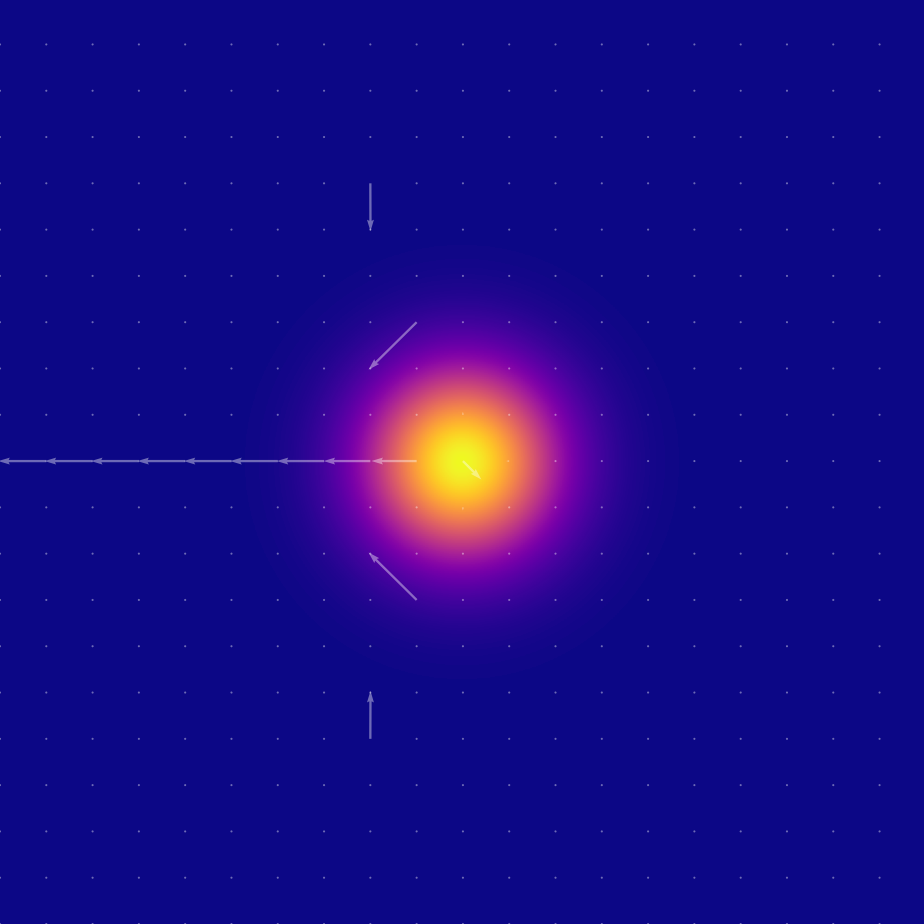
\includegraphics[width=0.48\textwidth]{figures/xi_electron_modulus_vector_overlay.png}
\caption{GCFT electron: a stable, left-chiral field knot in $\nabla \times \nabla \arg(\Xi)$. The persistent curl structure retains phase energy in a compressed coherence well.}
\label{fig:xi_electron_knot}
\end{figure}

\subsection{\texorpdfstring{Muon: Overcompressed $\Xi$ Core}{Muon: Overcompressed Xi Core}}

The muon represents a similar structure but exceeds the coherence comfort zone. Its overcompressed internal tension ($\sim$105\,MeV; $\sim$7.8 million luxions) causes rapid decay into a lower-energy state---typically into an electron and neutrinos. The decay pathway reflects the reconfiguration of phase tension into more stable knots.

\subsection{\texorpdfstring{Tau: Extreme Knot Instability}{Tau: Extreme Knot Instability}}

The tau lepton is an even more overcompressed $\Xi$-knot ($\sim$1.3$\times10^8$ luxions), so unstable that it rapidly unwinds, decaying into lighter leptons and neutrinos via the same decoherence logic.

\subsection{Neutrino: Pure Synchrony Mode}

The neutrino has no locked compression core. It is instead a mobile synchrony fluctuation---a coherence drift without compression. Because it lacks mass-locking, it interacts minimally and may oscillate via environmental phase realignment. Neutrinos are thus long-lived coherence shuttles~\cite{Hacquier2025a}.

\subsection{Lepton Resonance Table}

\begin{table}[H]
\centering
\begin{tabular}{lcccc}
\hline
\textbf{Particle} & \textbf{Mass (MeV)} & \textbf{Luxions} & \textbf{GCFT Topology} & \textbf{Stability/Decay} \\
\hline
Electron ($e^-$) & 0.511   & $\sim$37,573     & Stable $\Xi$-knot      & Stable \\
Muon ($\mu^-$)   & 105.7   & $\sim$7.8$\times 10^6$ & Compressed knot     & Rapid decay \\
Tau ($\tau^-$)   & 1776.9  & $\sim$1.3$\times 10^8$  & Overwound knot      & Very rapid decay \\
Neutrino ($\nu$) & $<0.0000022$ & $<$100    & Synchrony wave         & Oscillating \\
\hline
\end{tabular}
\caption{GCFT lepton mapping: All lepton masses arise from luxion compression and phase topology in the coherence field $\Xi$. Charge and decay follow from knot winding and curvature.}
\label{tab:lepton_gcft}
\end{table}

\subsection{Charge as Field Chirality}

GCFT redefines electric charge as a topological winding number:
\[
q = \frac{1}{2\pi} \oint_C \nabla \arg(\Xi) \cdot d\vec{\theta}
\]
Left-handed torsion corresponds to positive charge, right-handed to negative. The electron is a left-chiral $\Xi$-curl, while the positron is its mirror-symmetric torsion knot. Charge conservation becomes conservation of field chirality.

\subsection{Implications and Predictions}

Leptons in GCFT are not irreducible. They are the lowest-energy phase configurations that resist decoherence. Their behavior---including quantization, charge, and mass---follows from stability conditions in~$\Xi$, not from imposed quantum numbers or symmetry groups. This framework predicts coherence-driven phase transitions under compression or environmental decoherence, and allows for reinterpretation of lepton oscillation, charge inversion, and decay as topological transitions in the field.

\paragraph{GCFT Predictions:}
GCFT asserts that lepton charge and generation hierarchy are set by field topology; no stable leptons exist beyond the tau. The model also predicts subtle low-frequency $\Xi$-chirps preceding muon/tau decays, potentially detectable in high-precision decay experiments. Observation of any stable charged lepton heavier than the tau, or fractional lepton charge, would falsify this framework.

\subsection{Lepton Mixing and GCFT Topology}
\label{sec:lepton_mixing}

In GCFT, lepton generation transitions---such as muon-to-electron decay or neutrino flavor oscillations---arise not from fundamental mixing matrices, but from topological coupling between metastable Ξ-knot configurations. Each lepton corresponds to a quantized field structure with distinct phase tension, coherence retention time, and torsional symmetry. When coherence pressure, environmental curvature, or phase interference exceeds a critical threshold, a lepton can reconfigure into another topologically allowed state.

\paragraph{Flavor Oscillations:}
Neutrino oscillations are explained as slow, ambient transitions between mobile synchrony waves. Since neutrinos lack a mass-locked core, they remain sensitive to external coherence gradients and can phase-align with different oscillatory modes over macroscopic distances. The oscillation probability thus reflects the local topology of the Ξ-field rather than eigenstate superposition in a Hilbert space.

\paragraph{Effective Mixing:}
The CKM and PMNS matrices of the Standard Model~\cite{Pontecorvo1968} are reinterpreted in GCFT as effective tensors encoding the coupling likelihood between neighboring field topologies. For instance, muon-to-electron decay is modeled as a knot collapse where phase winding exceeds stability margin and redistributes coherence into a lower-tension configuration. CP asymmetries emerge from the chiral geometry of the $\Xi$-field during such transitions---particularly if the local torsion field $\nabla \times \nabla \arg(\Xi)$ is anisotropic.

\paragraph{Topological Constraints and Falsifiability:}
GCFT predicts that flavor transitions are not universal but topology-dependent: not all transitions are allowed, and certain configurations may be forbidden by field geometry. This imposes sharp constraints on decay modes and oscillation pathways. Detection of lepton flavor transitions that violate coherence-conserving topologies---e.g., stable heavy leptons beyond the tau, or non-symmetric neutrino mixing patterns at extreme coherence pressure---would falsify this formulation.

\paragraph{Experimental Link:}
Precision timing experiments, especially those measuring neutrino phase shift in varying gravitational or electromagnetic backgrounds, offer a direct test of GCFT's topological mixing logic. Deviations from standard PMNS predictions in such regimes could indicate environmental phase coupling, not mass eigenstate transitions.

